\documentclass[8pt]{article}
\usepackage{amsmath, xfrac, enumitem, graphicx, ulem, float, bigints, bm, textcomp}
\usepackage[margin=0.7in]{geometry}
\graphicspath{ {images/} }
\title{Strength of Materials GATE}\author{Kulasekaran}
\linespread{0.8}
\begin{document}
\maketitle
\begin{center}
	\section*{\uwave{1. Properties Of Materials}}
\end{center}
\dashuline{\textbf{Basics}}\\
	\begin{itemize}
		\item \textbf{Longitudinal Axis: }The Line passing through the center of all the planes along the longest dimension of the member is called as Longitudinal Axis. 
		\item \textbf{Cross Sectional Area (CS): }The plane normal to the longitudinal axis of the object
		\item \textbf{Prismatic Bar: }A member with constant cross-sectional area along its whole length
	\end{itemize}\hrulefill\\\\
%-----------------------------------------------------------------------------------------%
\dashuline{\textbf{Stress :-}}
	\begin{itemize}
		\item \textbf{Stress($\sigma$): }The internal resisting force which resists deformation in object when a force in acting on it. $\sigma = \dfrac{F}{A}$
		\begin{itemize}
			\item Stress is developed only when the motion due to the force is restricted
			\item Pressure and Stress are not the same. Pressure is external Normal force over a surface. 
			\item \textbf{Normal Stress($\sigma$): }Stress acting perpendicular to CS area.
				\begin{itemize}
					\item[] \textbf{Sign Convention:}
					\item Tensile stress ($\leftarrow\boxed{...}\rightarrow$) = Positive (+ve)
					\item Compressive stress ($\rightarrow\boxed{...}\leftarrow$) = Negative (-ve)
				\end{itemize}
			\item \textbf{Shear Stress($\tau$): }Stress acting tangential(parallel) to CS area.
		\end{itemize}
		\item \textbf{Engineering (or) Nominal Stress}
			\begin{itemize}
				\item[$\rightarrow$] $\boxed{\sigma_{Engg}=\dfrac{F}{A_0}}$
				\item[$\rightarrow$] $A_0$ = Original CS Area. Its called Original because, when an object is developing stress, there will be deformation to the object will change the cross sectional area. But, if we are using the initial cross sectional area to calculate stress, then its called Engineering stress (or) Nominal stress (or) \textbf{Average stress}
			\end{itemize}
		\item \textbf{True stress (or) Actual stress}
			\begin{itemize}
				\item[$\rightarrow$] $\boxed{\sigma_{actual} = \dfrac{F}{A_a}}$
				\item[$\rightarrow$] $A_a = A_0 + \Delta A$
					\begin{itemize}
						\item $\Delta A$ = +ve for Compression, as Area($\uparrow$) during compression
						\item $\Delta A$ = -ve for Tension, as Area($\downarrow$) during Tension
					\end{itemize}
			\end{itemize}
		\item[$\implies$] In Tension $\boxed{\sigma_{True} > \sigma_{actual}}$  \hspace{1cm}$\implies$In Compression $\boxed{\sigma_{True} < \sigma_{actual}}$ 
	\end{itemize}\hrulefill\\\\
%-----------------------------------------------------------------------------------------%
\dashuline{\textbf{Strain($\epsilon$) :-}}
	\begin{itemize}
		\item $\boxed{\epsilon=\dfrac{Change\;in\;dimension}{Original\;dimension}=\dfrac{\Delta L}{L}}\implies \boxed{\epsilon_{Engg}=\dfrac{\Delta L}{L_0}} \implies \boxed{\epsilon_{actual}=\dfrac{\Delta L}{L_a}} \impliedby \boxed{L_{a}=L_0\pm\Delta L}$
		\item $L_a=L_0+\Delta L$ for Tension \hspace{1cm}$L_a=L_0-\Delta L$ for Compression
		\item \textbf{Relationship between $\sigma_{Engg}\;\&\;\sigma_{actual}$ : }$\boxed{\sigma_{actual}=\sigma_{Engg}(1\pm\epsilon_{Engg})}\impliedby +ve(Tension)\;\&\;-ve(Compression)$
	\end{itemize}\hrulefill\\\\
%-----------------------------------------------------------------------------------------%
\dashuline{\textbf{Stress-Strain curve :-}}
	\begin{itemize}
		\item The Mechanical properties of materials used in engineering are determined using experiments performed on small specimens
			\begin{itemize}
				\item \textbf{ATSM} - American Society for Testing and Materials
				\item \textbf{UTM} - Universal Testing Machine (for Tension test)
				\item \textbf{Specimen spec} - Must be a cylindrical rod with L/D = 4
			\end{itemize}
		\item \textbf{Stress-Strain curve for Tension}
			\begin{itemize}
				\begin{figure}[H]
					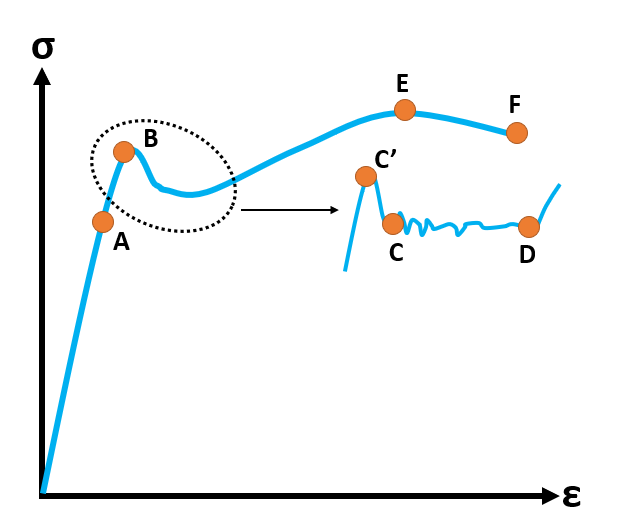
\includegraphics[scale=0.4]{stress-strain-curve.png}
					\centering
				\end{figure}
				\item \textsc{A = Proportional Limit}
					\begin{itemize}
						\item \textbf{Hooke's Law: } stress $\propto$ strain
						\item Hooke's law is valid upto this point i.e., Linear variation of stress and strain upto A
					\end{itemize}
				\item \textsc{B = Elastic limit}
					\begin{itemize}
						\item Maximum stress upto which material can retain its original dimension upon load removal
						\item Material behaves perfectly elastic up until B
						\item Only Elastic or Elastoplastic deformation (Elastoplastic = both plastic and elastic deformation)
					\end{itemize}
				\item \textsc{C' = Upper Yield Point}
				\item \textsc{C = Lower Yield Point}
				\item \textsc{CD = Perfectly Plastic Region}
				\item \textsc{DE = Strain Hardening Region}
				\item \textsc{E = Ultimate Yield Point}
				\item \textsc{F = Fracture Point}
			\end{itemize}
	\end{itemize}
\end{document}
